\chapter{Methodology}
\label{chap:methodology}

In this section, we present a methodology for performance evaluation of deep learning inference, specifically for edge and cloud inference.
To develop this methodology we make use of the best practices for performance evaluation by Ousterhout \cite{Ousterhout:2018:AMO:3234519.3213770} and Jain\cite{books/daglib/0076234}.


\begin{figure}[!htb]
\centering
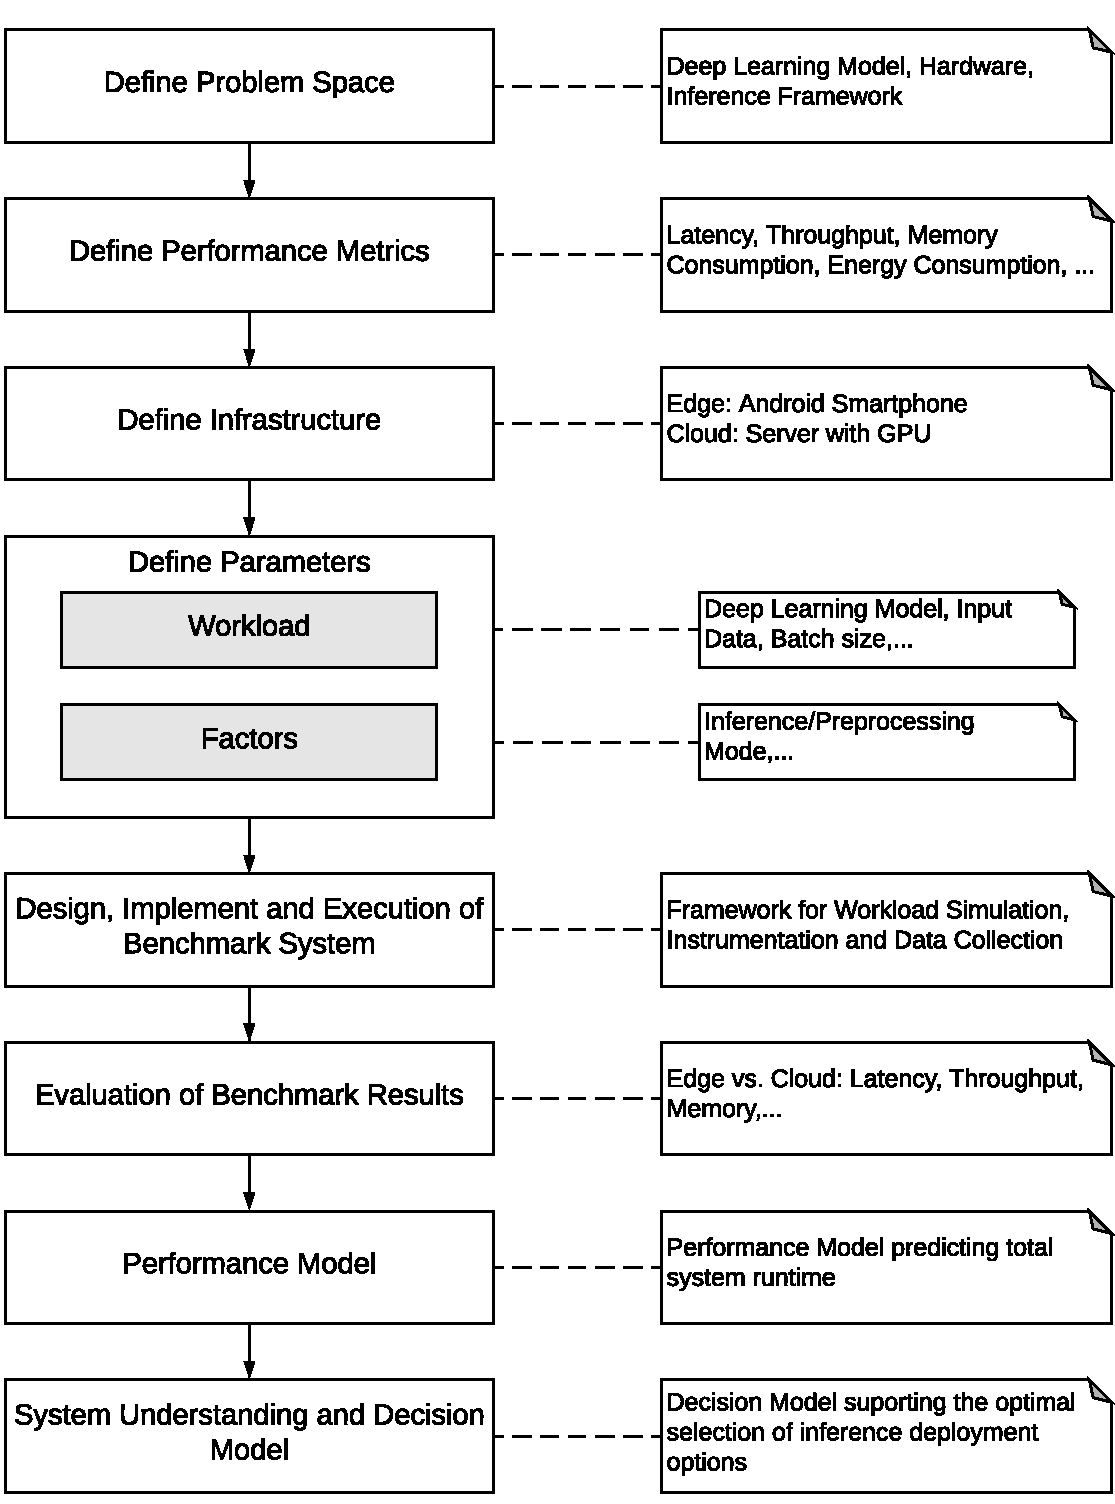
\includegraphics[width=0.7\textwidth]{./Bilder/Methodology.pdf}
\caption{Methodology for the performance evaluation of deep learning inference}
\label{fig:Methodology}
\end{figure}
To reach this goal, a systematic approach for performance evaluation is needed.
This methodology can be seen in figure \ref{fig:Methodology} and consists of a multiple-step process.


The goal of the performance evaluation is to get a better understanding of deep learning inference, specifically the trade-offs between edge and cloud inference.
Based on this understanding we can, in the last step, propose a decision model, that helps in the decision, whether a deep learning model should be deployed to the edge, to a cloud-backend or is not feasible for deployment at all.


To model the performance of deep learning inference, it is crucial to understand the underlying problem space in the first place.
Understanding the system boundaries helps to choose the correct performance metrics, workloads and parameters affecting performance.
Therefore the topic of deep learning in general, but specifically inference and the deployment of deep learning models on both edge and cloud-backends have to be studied.

Based on the understanding of the problem space performance metrics, critical for assessing the inference performance of a system, can be derived.

We will use measurements as the evaluation technique of this thesis. 
Therefore we have to develop a benchmark framework supporting a use case, that is used as an exemplary system helping to illustrate the trade-offs between edge and cloud inference for better system understanding.

Therefore the next steps towards such a benchmark framework are to select an infrastructure, that is representative of real-life conditions to achieve applicable measurements. 
This infrastructure consists of hardware components and frameworks supporting this hardware. 

The next step is to define the parameters to be studied, which all affect performance.
There can be differentiated between two types of parameters, workloads and factors.
Factors are parameters of the system with various levels, that will be varied in the evaluation. An example factor would be if the inference is performed at the edge or the cloud-backend.
Workloads are requests to the system, in our case a deployed deep learning model, by a user.
This requests can come in different shapes, thus having a different impact on performance.



After defining the infrastructure, parameters and performance metrics, the benchmark framework can be implemented as a framework for handling workload simulation, performance metrics instrumentation and data collection of the measurements.
This system then can be used to generate the benchmarks. 

Afterwards, the collected measurements can be used for evaluation and interpretation.
Depending on the results of the evaluation concrete recommendations can be given for the optimal deployment option in regard to the benchmarked infrastructure and workload.

Next, we use the collected benchmarks to create a performance model, predicting the system run-time including preprocessing, inference and network latencies for a given system configuration.
These predictions then can be used to generate recommendations for the optimal deployment option.

Finally, the knowledge from the previous steps can be generalized to create a decision model for the optimal selection of deployment options for deep learning inference.
This decision model can be applied to all decision processes where deep learning models have to deployed for real-time AI applications, independent of deep learning model architecture, workload, infrastructure or framework.



\vspace{0.5cm}
In the next section, we instantiate the presented methodology step by step.



%In order to model the performance of deep learning inference, it is crucial to understand the underlying problem space. 
%In section \ref{chap:fundamentels} we presented the fundamentals of Deep Learning Models, their deployment and the frameworks needed to perform the inference.







\endinput 